\documentclass{article}
\usepackage{amsmath}
\usepackage{amssymb}
\usepackage{amsthm}
\usepackage{thmtools}
\usepackage{cases}
\usepackage{enumitem}
\usepackage{xcolor}
\usepackage{cancel}
\usepackage{cite}
\usepackage{graphicx}
\usepackage{float}
\usepackage{array}
\usepackage{multirow}

\usepackage{algorithm2e}
\RestyleAlgo{ruled}
\SetKwComment{Comment}{/* }{ */}

\usepackage{geometry}
\geometry{margin=4cm, vmargin=3cm}

\setlength\parindent{0pt}

\title{Asian options pricing}
\author{David Castro \qquad Maxime Leroy}
\date{15 Januray 2024}

\begin{document}
\maketitle

\section*{Introduction}

An Asian option is any option with payoff of the form:
\[
	\left( S_t \right)_{t \in [0, T]} \mapsto g \left( S_T, A_T \right) \quad \text{with} \quad A_T := \frac{1}{T} \int_0^T S_u du
\]
where $\left( S_t \right)_t$ denotes the trajectory of the underlying and $T$ is the maturity of the option.
For instance, a \textit{fixed-strike} Asian call has $g(x, a) := e^{-rT} \left[ a - K \right]_+$ where $K$ denotes the strike
and a \textit{floatting-strike} Asian call has $g(s, a) := e^{-rT}  \left[ s - a \right]_+$.
In the first case, the option is exercised by its owner
if the underlying has lied above the strike \textbf{on average} throughout its lifetime. In the second case,
it is worth exercising it when the underlying is above its average value at expiry.

\

This work studies different pricing techniques for Asian options and will tackle \textbf{only fixed-strike Asian calls}
for simplicity. Furthermore, we will use Black-Scholes model. In that context, simulating $S_T$ is straightforward
and the real challenge consists in simulating $A_T$. That is why our developments for fixed-strike Asian calls
adapt directly to any Asian option of the form given above.

\

We first introduce and implement different Monte-Carlo approaches as developed by Lambert et al. \cite{main}
and B. Bouchard \cite{Bouchard}. We then compare them with a PDE approach as presented by
Rogers et al. \cite{Rogers}.

\section*{Assumptions and notations}

We consider the case of an arbitrage-free complete market and note $\mathbb Q$ the corresponding
risk-neutral measure. Therefore, the true price of the option is given by:
\[
	C := e^{-rT} \mathbb E_{\mathbb Q} \left[ [ A_T - K ]_+ \right]
\]
where $r$ is the risk-free interest rate, assumed to be constant.
As specified above, we also use Black-Scholes model, which yields:
\begin{equation}
	\forall t \in [0, T], \ S_t = S_0 \exp \left\{ \left( r - \frac{\sigma^2}{2} \right) t + \sigma W_t \right\}
	\tag{BS}
\end{equation}
where $W := (W_t)_{t \in [0, T]}$ denotes a Wiener process under $\mathbb Q$.

\

In the context of Monte-Carlo methods, we call \textbf{a scheme} a random variable $\bar A_T$ made to approximate
the quantity $A_T$ for a given set of parameters. Therefore, provided $\{ \bar A_T^i \}_{i = 1, \dots, n}$ are
independent and identically distributed (i.i.d.) copies of $\bar A_T$, the Monte-Carlo estimate of the fixed-strike
Asian call we get is:
\[
	\theta_n := e^{-rT} \sum_{i=1}^n \left[ \bar A_T^i - K \right]_+ \xrightarrow[n \to \infty]{\mathbb P}
	e^{-rT} \mathbb E_{\mathbb Q} \left[ [ \bar A_T - K ]_+ \right]
\]

For $m \in \mathbb N^*$ time steps, we note:
\begin{itemize}[label=$\cdot$]
\item $t_0, \dots, t_m$ the regular subdivision of $[0, T]$, whose mesh is thus $h = \frac{T}{m}$.
\item $\bar W_{t_0}^m, \dots, \bar W_{t_m}^m$ a realization of $W$ at these time steps.
\item $\bar S_{t_0}^m, \dots, \bar S_{t_m}^m$ the corresponding realization of the underlying, obtained
	with (BS).
\item $\mathcal B_h$ the $\sigma$-field generated by $\left\{ S_{t_0}, \dots, S_{t_m} \right\}$.
\end{itemize}

\section{Naive approach}

The most basic Monte-Carlo approach to the problem consists in approximating the integral
of the underlying over its trajectory by a Riemann sum. This is our first scheme:
\begin{equation}
	A_T \approx \bar A_T^{r, m} := \frac{h}{T} \sum_{k=0}^{m-1} \bar S_{t_k}^m
	= \frac{1}{m} \sum_{k=0}^{m-1} \bar S_{t_k}^m 
	\tag{1}
\end{equation}

Figure 1 shows the result
of this method for different values of $K$, $T$ and $\sigma$ where we took $n =10,000$ and $m=100$.
One can already notice that it tallies with the common idea that Asian calls are cheaper than European calls
for a given set of parameters. Also, quite intuitively, the gap widens when $\sigma$ and $T$ grow: the smaller
both of them are, the closer to the initial value the underlying will remain, leading to $A_T \approx S_T \approx S_0$
on average.

\begin{figure}[H]
  \hspace*{-0.02\linewidth}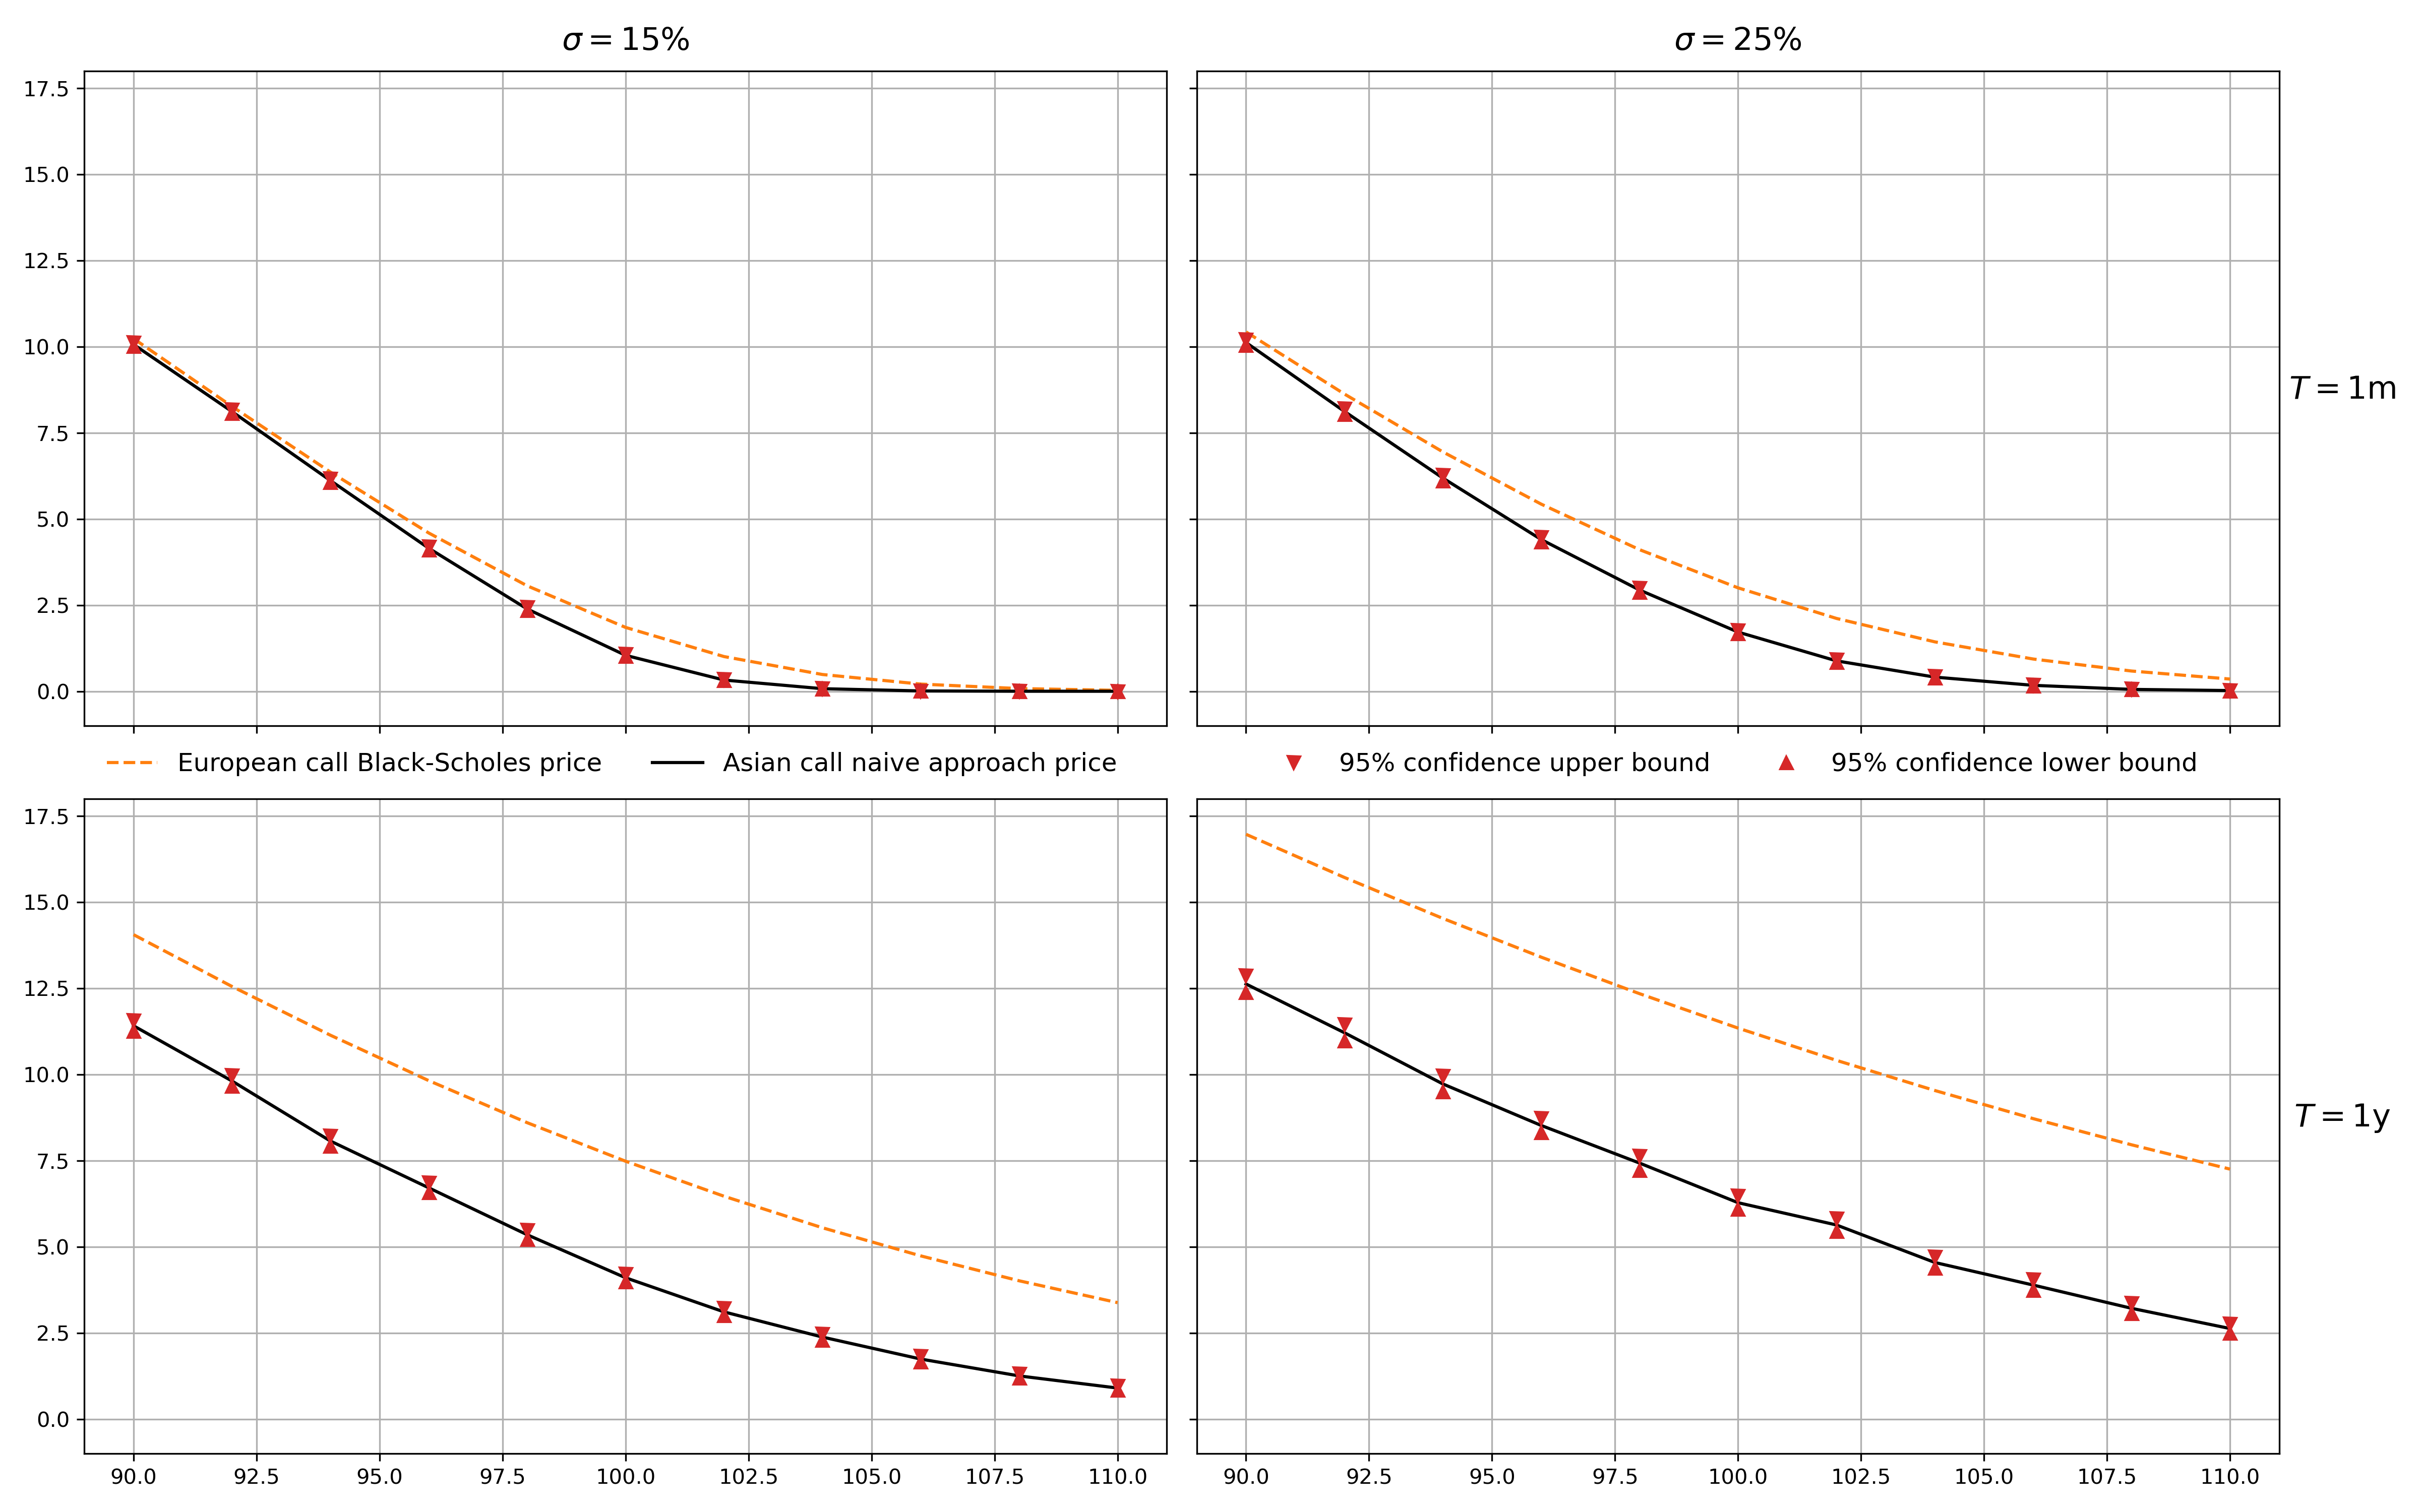
\includegraphics[width=1.065\textwidth]{charts/prices.png}
  \caption{Fixed-strike Asian call naive pricing for different values of $K$, $\sigma$ and $T$}
\end{figure}

However, these charts, particularly the one for $\sigma = 25\%$ and $T=1$y, reveal some fluctuations with
a greater magnitude than the length of the $95\%$ confidence intervals plotted in red. This stems from the bias
introduced by the approximation of $A_T$. This seems to be the main flaw of the
naive approach: even if the variance already looks satisfactory, the bias increases rapidly with the parameters, which
yields imprecise results.

\

The following models all give similar charts. In the below, we rather focus on the graphical representation
of the convergence properties of each scheme. As suggested in the previous paragraph, this is
the main challenge that the following approaches mean to address.

\section{Improved Monte-Carlo approaches}
\subsection{Two finer approximations}

A first improvement of the above approach proposes to better use the information provided by the simulation
$\bar S_0^m, \bar S_{t_1}^m, \dots, \bar S_T^m$ to approximate the integral $A_T$.
It relies on the fact that once the trajectory has been simulated, the best estimation of the price is:
\[
	\bar C^m := e^{-rT} \mathbb E \left[ \left[ A_T - K \right]_+ \mid \mathcal B_h \right]
\]

By the tower property, the expectation (estimated by a Monte-Carlo method with $n$ trajectories)
of this conditional expectation is the price of the Asian call.
At this stage, this quantity is not known either. \cite{main} introduces the following simplification (S):

\begin{align}
	\bar C^m &\approx e^{-rT}  \bigl[ \mathbb E \left[A_T
		\ \vert \ \mathcal B_h \right] - K \bigr]_+
	\tag{S} \\
	&= e^{-rT} \left[ \frac{1}{T}\sum_{k=0}^{m-1} \mathbb E \left[ \int_{t_k}^{t_{k+1}} S_u du
		\ \Big\vert \ \mathcal B_h \right] - K \right]_+
	\notag \\
	&= e^{-rT} \left[ \frac{1}{T}\sum_{k=0}^{m-1} \int_{t_k}^{t_{k+1}} \mathbb E \left[ S_u
		\ \big\vert \ \mathcal B_h \right] du - K \right]_+
	\notag \\
	&= e^{-rT} \left[ \frac{1}{T}\sum_{k=0}^{m-1} \bar S_{t_k}^m \int_{t_k}^{t_{k+1}}
		\mathbb E \left[ e^{\left( r - \frac{\sigma^2}{2} \right) (u - t_k) + \sigma \left( W_t - W_{t_k} \right)}
		\ \big\vert \ \mathcal B_h \right] du - K \right]_+
	\notag
\end{align}

We need to further simplify this expression. Let us considere the function $f$ defined as:
\[
	f : (t, w) \mapsto \exp \left\{ \left( r - \frac{\sigma^2}{2} \right) t + \sigma w \right\}
\]
A first-order Taylor expansion gives (by It\^o's lemma):
\[
	f(t, W_t) \underset{t \to 0}{\approx} 1 + \partial_t f(0, 0) t + \partial_w f(0, 0) W_t
	+ \frac{1}{2} \partial_{ww}^2 f (0, 0) t = 1 + rt + \sigma W_t
\]

It leads to the additional approximation below for all $k \in \{ 0, \dots, m - 1 \}$:
\[
	\int_{t_k}^{t_{k+1}} \mathbb E \left[ S_u \mid \mathcal B_h \right] du
	\approx \bar S_{t_k}^m \int_{t_k}^{t_{k+1}}
		\mathbb E \left[ 1 + r (u - t_k) + \sigma \left( W_t - W_{t_k} \right)
		\ \big\vert \ \mathcal B_h \right] du
\]

Finally, the process
$\left\{ \left( W_u \mid \bar W_{t_k}^m, \bar W_{t_{k+1}}^m \right) ; u \in [t_k, t_{k + 1}] \right\}$
follows a Brownian bridge, which allows
to compute the expectation and then the integral and yields the following scheme:

\begin{equation}
    A_T \approx \bar A_T^{e, m} = \frac{1}{m} \sum_{k=0}^{m-1} \bar S_{t_k}^m
    	\left( 1 + \frac{rh}{2} + \sigma \frac{\bar W_{t_{k+1}}^m - \bar W_{t_k}^m}{2} \right) \tag{2}
\end{equation}

The above development is actually equivalent to a trapezoidal method in comparison with the more
basic Riemann sum used in scheme $(1)$.

\

Instead of simplification (S), \cite{Bouchard} and \cite{main} suggest a quite similar approach. For each step
of the Monte-Carlo estimation, first fix a trajectory with the explicit formula given by Black-Scholes model
(same as before). Then, rather than computing the conditional expectation $\bar C^m$, simulate a realization of
$e^{-rT} \left[ A_T - K \right]_+$ conditionally to the trajectory. Similarly:
\begin{align*}
	\int_{t_k}^{t_{k+1}} S_u du
	&\approx
	S_{t_k} \int_{t_k}^{t_{k+1}} \left\{ 1 + r (u - t_k) + \sigma \left( W_u - W_{t_k} \right) \right\} du \\
	&= h S_{t_k} \left\{ 1 + \frac{rh}{2} + \frac{\sigma}{h} \int_{t_k}^{t_{k+1}} \left( W_u - W_{t_k} \right) du \right\}
\end{align*}

Furthermore, the remaining integral of the increment of the Brownian Motion is a Gaussian variable and we can
compute its expectation and variance conditionally to the trajectory since the integrand follows a Brownian Bridge.
Thus, we can indeed simulate it as stated above. In the following, we note:
\[
	\bar I_k^m := \left( \frac{1}{h}
	\int_{t_k}^{t_{k+1}} \left( W_u - W_{t_k} \right) du \ \Big\vert \ \mathcal B_h
	\right)
\]

In short, $\bar I_k^m \sim \mathcal N(\mu_k, \sigma_k^2)$ with the following parameters:
\begin{align*}
	\mu_k
	&= \frac{1}{h} \int_{t_k}^{t_{k+1}} \mathbb E \left[ W_u - W_{t_k} \mid \bar W_{t_{k+1}}^m, \bar W_{t_k}^m \right] du \\
	&= \frac{1}{h} \left( \bar W_{t_{k+1}}^m - \bar W_{t_k}^m \right) \int_{t_k}^{t_{k+1}} \frac{u - t_k}{t_{k+1} - t_k} du \\
	&= \frac{1}{2} \left( \bar W_{t_{k+1}}^m - \bar W_{t_k}^m \right)
\end{align*}
Interchanging the conditional expectation and the integrals yields:
\[
	\sigma_k^2 = \frac{1}{h^2} \int_{t_k}^{t_{k+1}} \int_{t_k}^{t_{k+1}}
		\mathrm{Cov} \left( W_u, W_v \mid \bar W_{t_{k+1}}^m, \bar W_{t_k}^m \right) du dv 
\]

\noindent Then, by symmetry of the covariance, we have:
\begin{align*}
	\sigma_k^2 &= \frac{2}{h^2} \int_{t_k}^{t_{k+1}} \left( \int_{t_k}^{v}
		\mathrm{Cov} \left( W_u, W_v \mid \bar W_{t_{k+1}}^m, \bar W_{t_k}^m \right) du \right) dv 
	 \\
	&= \frac{2}{h^2} \int_{t_k}^{t_{k+1}} \left( \int_{t_k}^{v} \frac{(t_{k+1} - v)(u - t_k)}{t_{k+1} - t_k} du \right) dv \\
	&= \frac{1}{h^2} \int_{0}^{h} \frac{h - v}{h} \left( \int_{0}^{v} 2u du \right) dv \\
	&= \frac{1}{h^3} \int_{0}^{h} (h - v) v^2 dv \\
	&= \frac{h}{12}
\end{align*}

The above finally yields the following scheme:

\begin{equation}
    A_T \approx \bar A_T^{p, m} = \frac{1}{m} \sum_{k=0}^{m-1}
    	\bar S_{t_k}^m \left( 1 + \frac{rh}{2} + \sigma \bar I_k^m \right) \tag{3}
\end{equation}

Considering the value of $\mu_k$, one can note this scheme is the same as the previous one except the fact
that (3) adds a random term with distribution $\mathcal N(0, \frac{h}{12})$ in the multiplicative factor.
To put it differently, in comparison with (3), (2) approximates $\bar I_k^m$ by its mean.

\

\begin{algorithm}[H]
\caption{Scheme (3) implementation}
\KwData{$n$ (number of independent simulations), $m$ (number of time steps)}
\KwResult{Estimation and $95\%$ confidence interval}
\For{$i = 1, \dots, n$}{
	Simulate $\bar W^{m, i}$\;
	Deduce $\bar S^{m, i}$ using Black-Scholes formula\;
	\For{$k=0, \dots, m - 1$}{
		Simulate $\bar I_k^{m, i}$ (conditionally to $\bar W^{m, i}$)\;
	}
	Compute $\bar A_T^{m, i}$ with $\bar S^{m, i}$, $\bar W^{m, i}$ and $\bar I_0^{m, i}, \dots, \bar I_{m-1}^{m, i}$\;
}
Compute the mean and standard error of the prices given by $\bar A_T^{m, 1}, \dots, \bar A_T^{m, n}$\;
\Return{the MC estimate and $95\%$ confidence interval for the price}\;
\end{algorithm}

\subsection*{Convergence analysis}

Before going further, we suggest comparing the results given by schemes (1)-(3).
Noticing that for a given strike $K$,
$a \mapsto [ a - K ]_+$ is $1$-lipschitz, we have for any scheme $\bar A_T$ that yields price $\widetilde C$
(ie, the price if we were able to compute the expectation exactly):
\[
	\vert \widetilde C - C \vert^2
	\leqslant e^{-2rT} \mathbb E_{\mathbb Q} \left[ \vert [ A_T - K ]_+ - [ \bar A_T^m - K ]_+ \vert^2 \right]
	\leqslant \mathbb E_{\mathbb Q} \left[ \vert A_T - \bar A_T^m \vert^2 \right]
\]

\noindent Consequently, in the context of fixed-strike Asian calls, the time step error is bounded
by the bias due to the approximation of $A_T$. This provides the following:
\begin{enumerate}[label=(\roman*)]
\item The bias of scheme $1$ is in $O \left( \frac{1}{m} \right)$.
\item The bias of scheme $2$ is in $O \left( \frac{1}{m} \right)$ with a lower constant than for scheme 1.
\item The bias of scheme $3$ is in $O \left( \frac{1}{m\sqrt{m}} \right)$.
\end{enumerate}

\noindent On the other hand, the Monte-Carlo error is in $O \left( \frac{1}{\sqrt{n}} \right)$ as usual.

\subsection*{Numerical results}

The numerical results, as shown in Figure 2, illustrate the bias provided above for each scheme.
They graphically confirm the obtained convergence speeds.

\begin{figure}[h]
  \hspace*{-0.025\linewidth}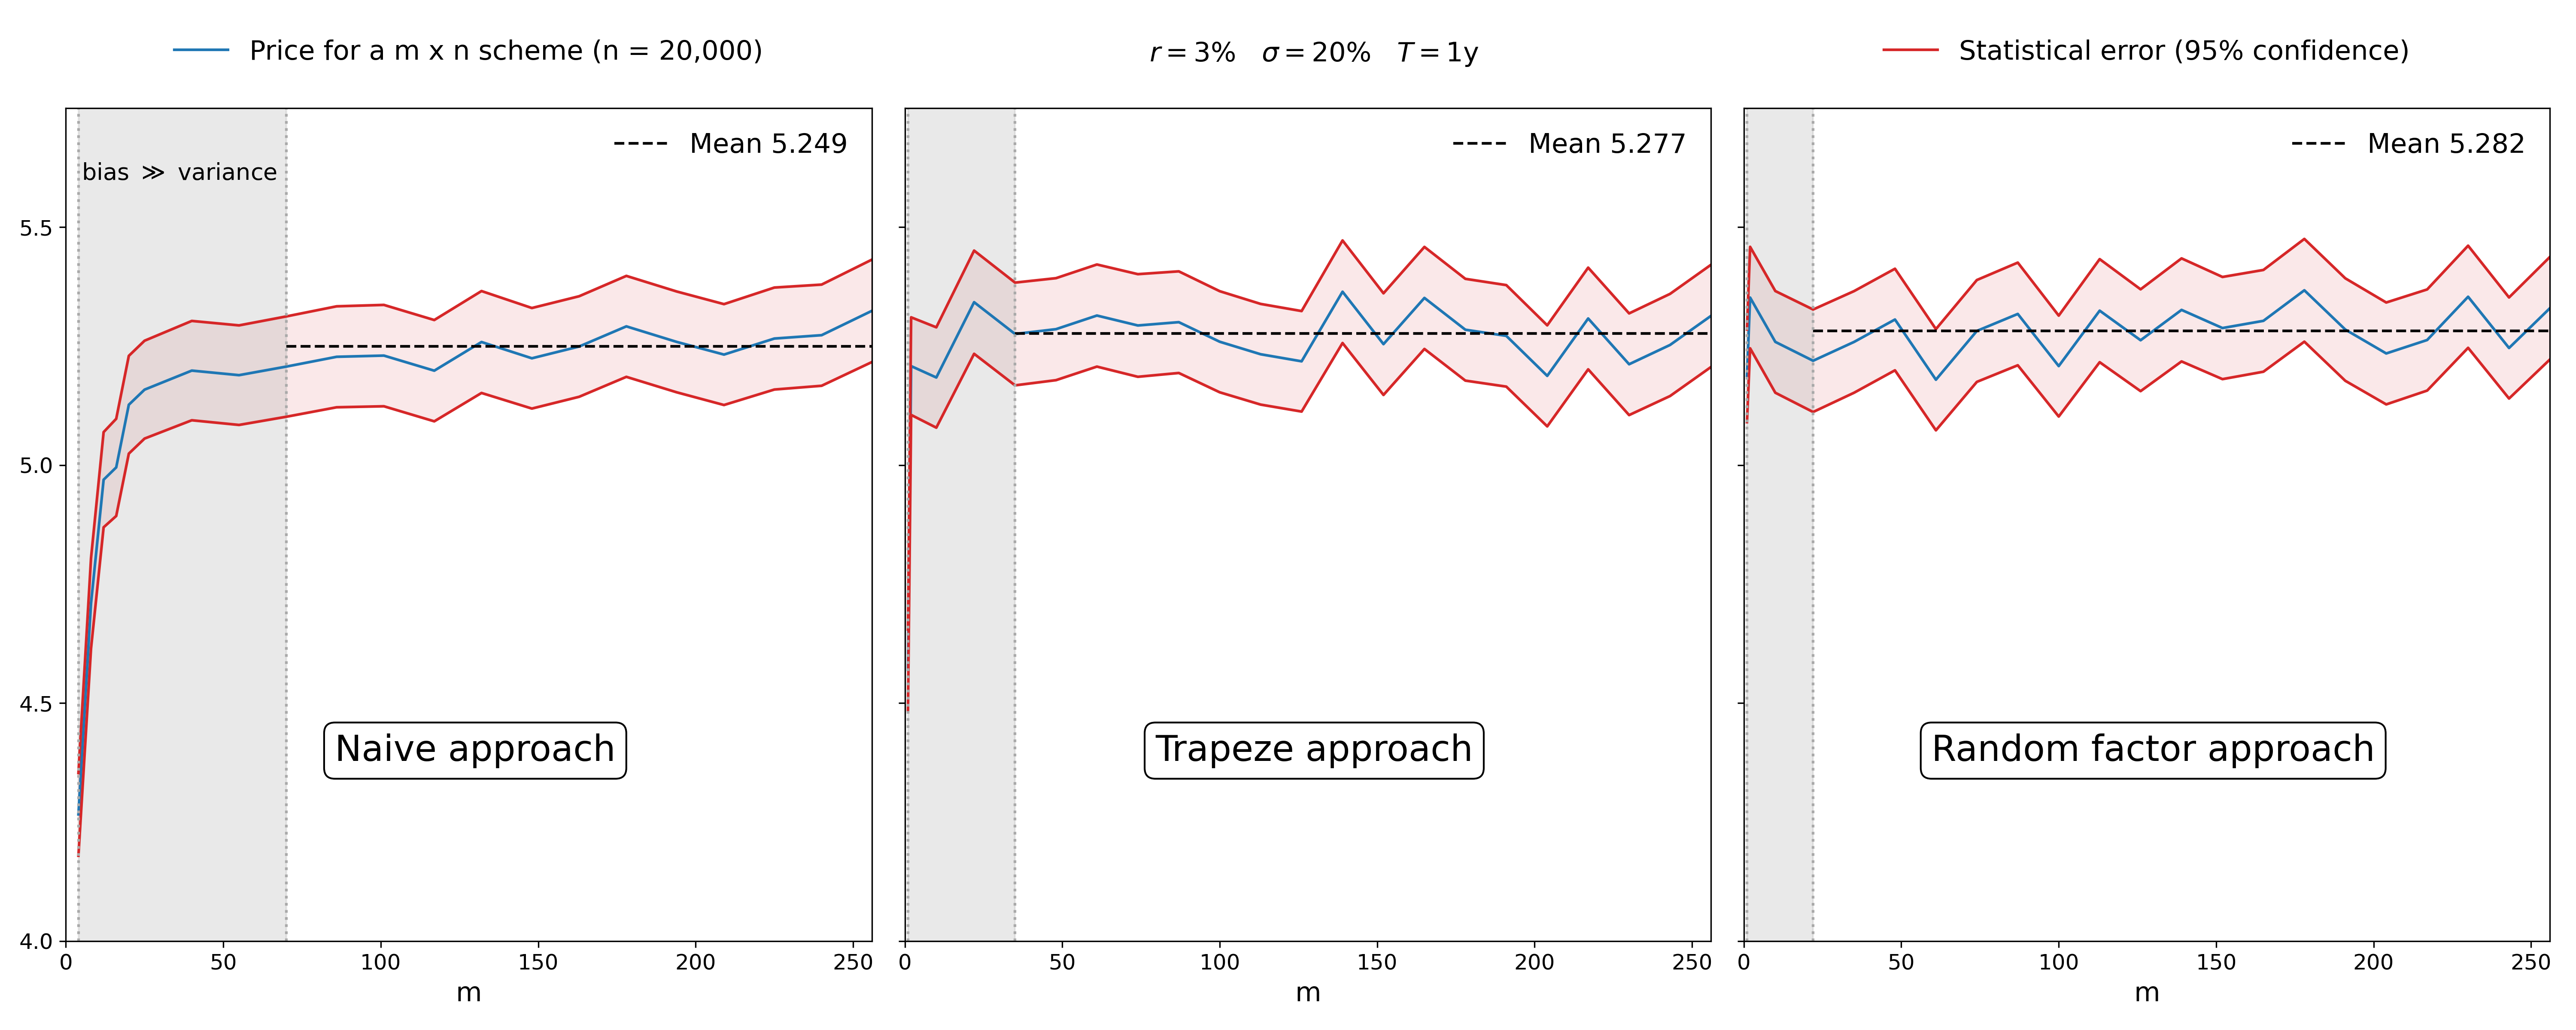
\includegraphics[width=1.04\textwidth]{charts/cvgce_wo_control.png}
  \caption{Convergence of schemes (1)-(3) for different values of $m$}
\end{figure}

\

Figure 2 shows the $95\%$ confidence intervals given by the three methods for fixed $n$ and $m$
varying up to $256$. As we do not have an analytical solution, it is difficult to compare the impact of the variance and that
of the bias by comparing the error to the confidence intervals for different values of $m$. However, since the proposed
methods are asymptotically unbiased, the black dotted lines are good approximations of the solution and we
can compare the fluctuations of the blue line with the width of the confidence intervals, in red. In the grey area,
that is to say for low values of $m$, the bias is high compared to the variance. For greater values of $m$, a plateau
seems to be reached and the observed deviations are mainly caused by the variance (the bias becomes negligible).
Thus, these charts allow
to choose $m$: the one at the edge of the grey zone is the most computationally-effective one that offers a satisfactory
level of accuracy. As explained before, there is actually no point in choosing higher values of $m$ since the decrease in
the bias would be hidden by the variance. Consequently, one can already notice the advantage of the two improved
methods on the right-hand side in comparison with the naive approach: $m$ can be chosen to be significantly lower
while achieving as good results. They allow better time complexity. Note however that their space complexity is worse.
In particular, the third method requires to simulate an additional $n \times m$ matrix of independent, normally
distributed coefficients.

\subsection{The use of a control variate}

The two improvements introduced in the above tackle the bias, which they successfully reduce for low values of $m$.
In order to improve the convergence speed with respect to parameter $n$,
Lambert et al. \cite{main} finally propose a variance reduction technique
for the three schemes above. It uses a control variate as introduced by Kemna et al. \cite{Vorst}.

\begin{equation}
	\theta_n = \sum_{i=1}^n \left( e^{-rT} \left[ A_T^i - K \right]_+ + \beta \left( Z^i - \mathbb E [Z] \right) \right)
	\tag{$\ast$}
\end{equation}

Observing that $e^x \approx 1 + x$ and $\ln(1 + x) \approx x$ when $| x |$ is small,
the idea relies on the approximation:
\[
	A_T = \frac{1}{T} \int_0^T S_u du \approx \exp \left\{ \frac{1}{T} \int_0^T \ln S_u du \right\}
	= S_0 \exp \left\{ \frac{1}{T} \int_0^T \ln \frac{S_u}{S_0} du \right\}
\]
The equality on the right-hand side justifies the validity of such approximation: if $r$ and $\sigma$ are small,
$S_u$ can be expected to remain near $S_0$ and $\ln \frac{S_u}{S_0} \ll 1$.
Therefore, we would like to use the following as a control variate in the case of a fixed-strike Asian call:
\[
	Z
	= e^{-rT} \left[ S_0 \exp \left\{ \left( r - \frac{\sigma^2}{2} \right) \frac{T}{2} +
		\frac{\sigma}{T} \int_0^T W_u du \right\}
		- K \right]_+
\]

Note that we can indeed compute the exact expression of $\mathbb E[Z]$. First, It\^o's lemma
gives $d(tW_t) = tdW_t + W_tdt$ and:

\[
	\frac{1}{T} \int_0^T W_u du = \frac{1}{T} \int_0^T (T-s) dW_s \sim \mathcal N \left(0, \frac{T}{3} \right)
	\quad \text{because} \quad \int_0^T (T-s)^2 ds = \frac{T^3}{3}
\]

If we note $a := \left( r - \frac{\sigma^2}{2} \right) \frac{T}{2}$, $b := \sigma \sqrt{\frac{T}{3}}$, $\rho :=\frac{K}{S_0}$,
$x^\ast := \frac{\ln \rho - a}{b}$ and $N$ the c.d.f of $\mathcal N (0, 1)$ then:
\begin{align*}
	\frac{\mathbb E[Z]}{e^{-rT} S_0}
	&= \int_{x^\ast}^{+ \infty} \left( e^{a + bx} - \rho \right) N'(x) dx \\
	&= e^{a + \frac{b^2}{2}} \int_{x^\ast - b}^{+ \infty} N'(u) du - \rho \int_{x^\ast}^{+ \infty} N'(x) dx
	\quad \text{with} \quad u = x - b \\
	&= e^{a + \frac{b^2}{2}} N(b - x^\ast) - \rho N(-x^\ast)
\end{align*}
	
On can check that the same computations yield Black-Scholes formula for the price of a European call.
Thus, we have the analytical expression. We finally need to provide a way to simulate the control variate $Z$
in each scenario. We define:

\begin{equation}
	\bar Z^{e, m} = e^{-rT} \left[ S_0 \exp \left\{ \left( r - \frac{\sigma^2}{2} \right) \frac{T}{2} +
		\frac{\sigma}{m} \sum_{i=0}^{m-1} \bar W_{t_k}^m \right\} - K \right]_+
	\tag{$i$}
\end{equation}

Plugging $\bar A_T^{e, m}$ from scheme $(1)$ and $\bar Z_T^{e, m}$ in $(\ast)$ yields a new estimator:
\begin{equation}
	e^{-rT} \left[ \bar A_T^{e, m} - K \right]_+ + \hat\beta_r \left( \bar Z_T^{e, m} - \mathbb E [Z] \right)
	\tag{4}
\end{equation}
where $\hat\beta_e$ is estimated with the empirical covariance of the variables.

\begin{figure}[H]
  \hspace*{-0.1\linewidth}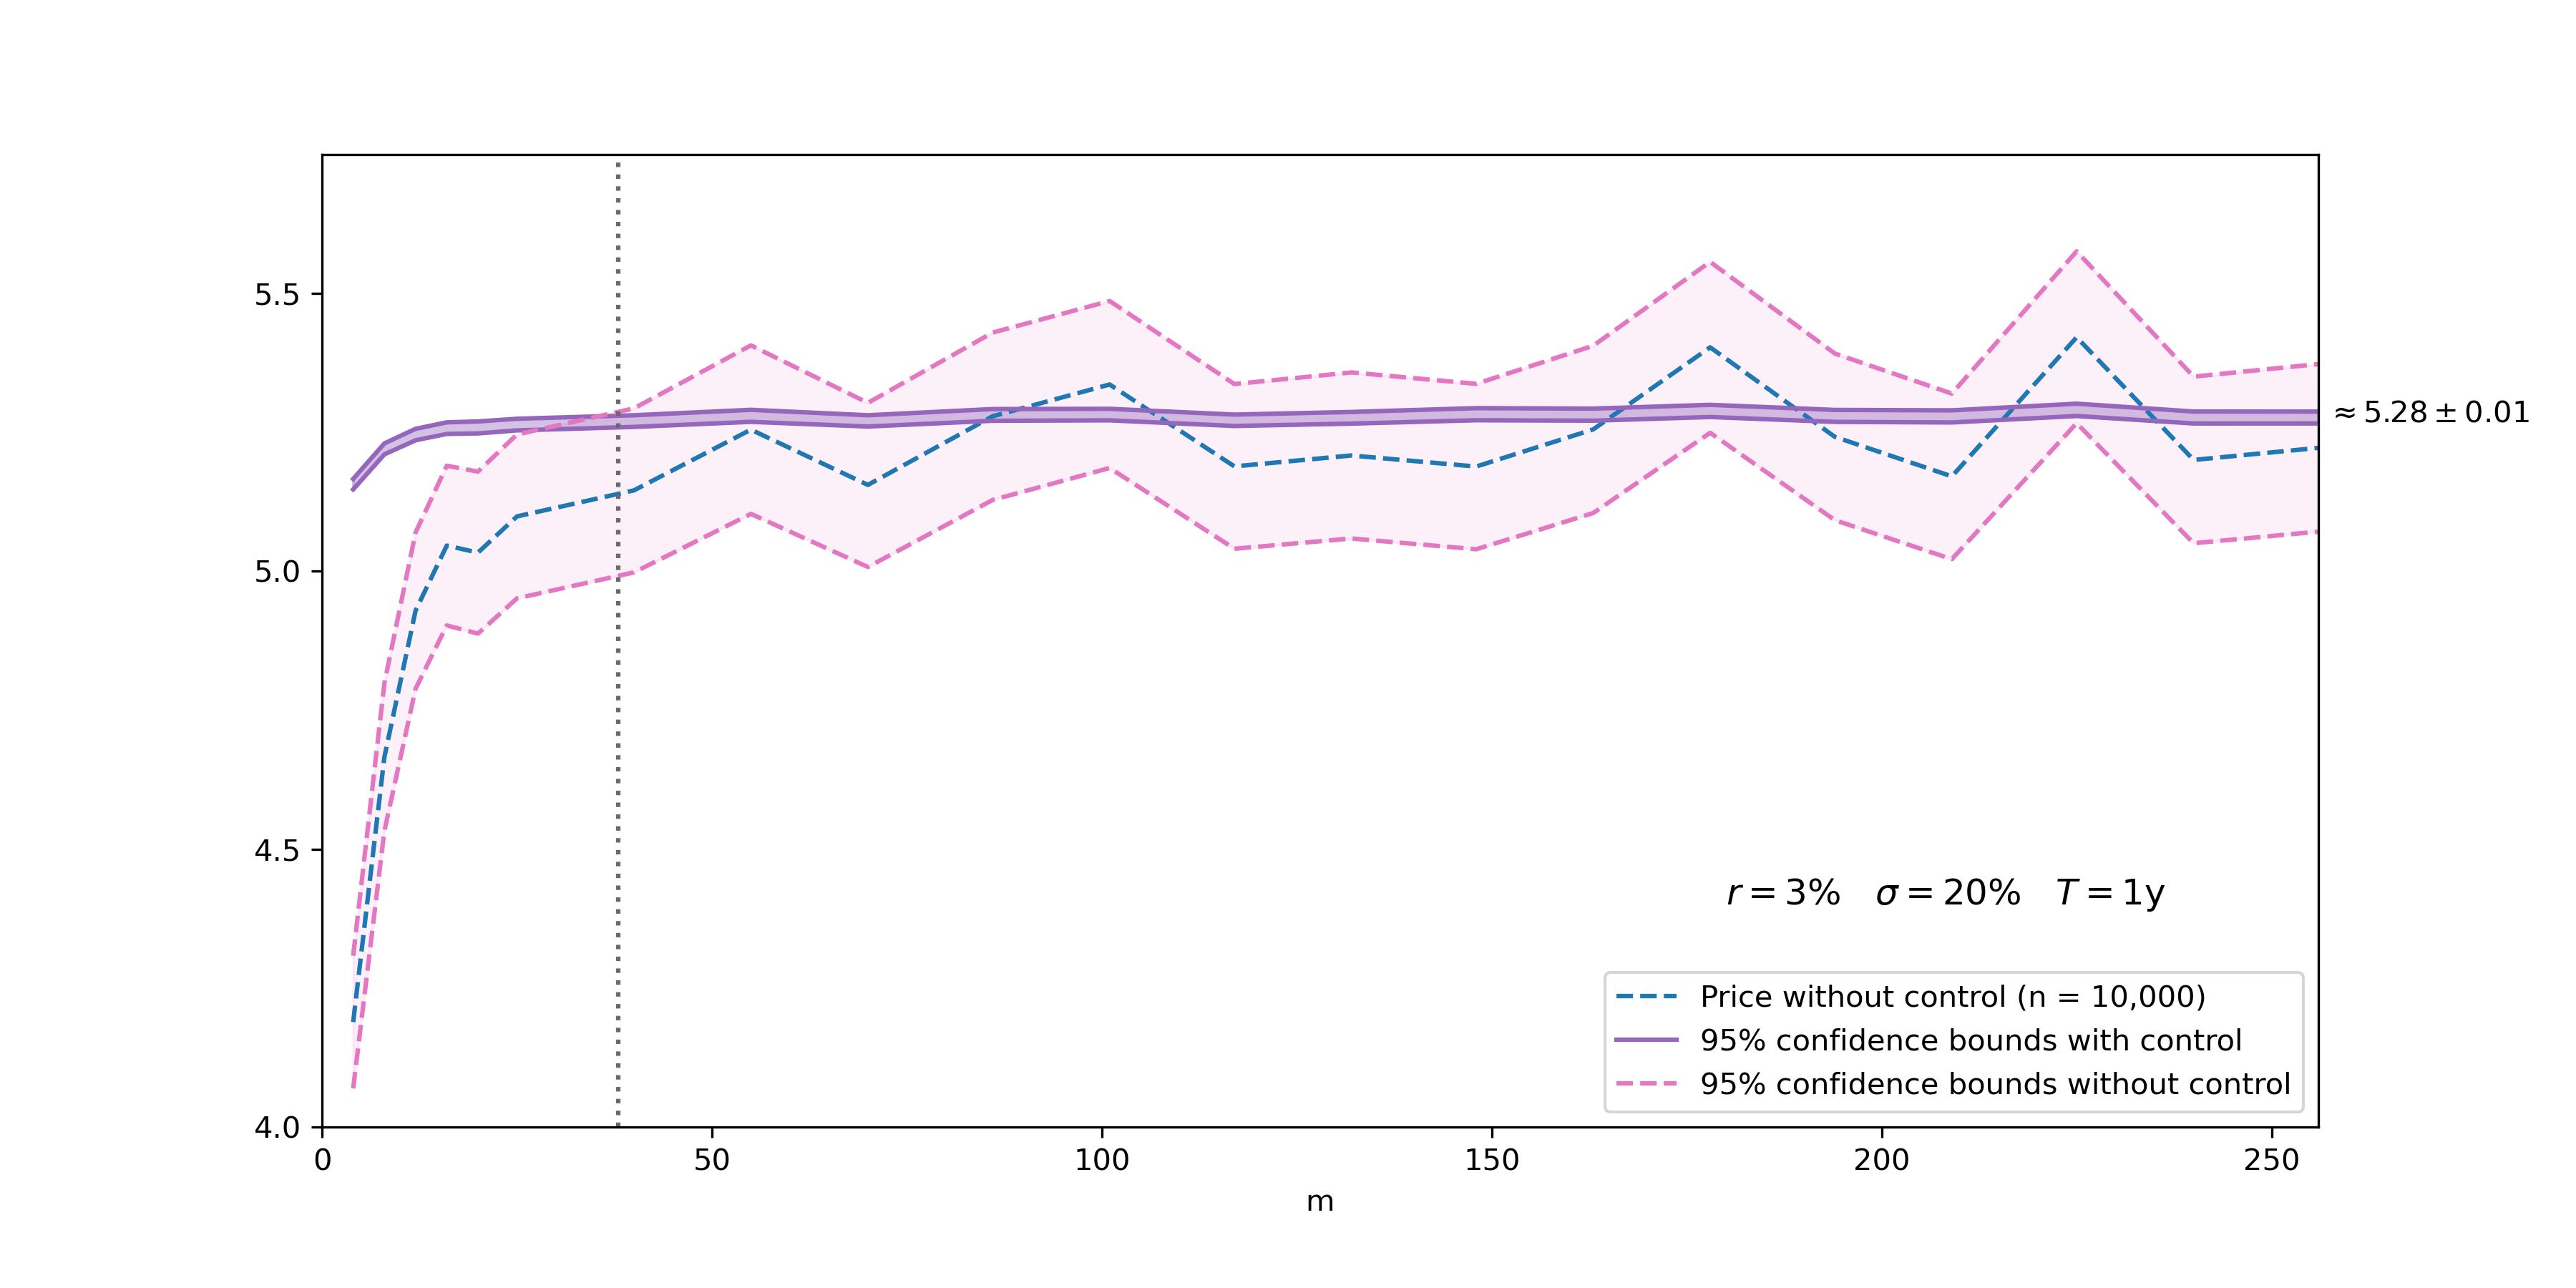
\includegraphics[width=1.1\textwidth]{charts/cvgce_control.png}
  \caption{Convergence of scheme (4) for different values of $m$}
\end{figure}

As expected, the statistical error (ie: the width of the confidence interval) is much more narrow. With this set of
parameters, it is about ten times smaller. The result is quite impressive. Besides, it does not only allow to take
a lower $n$ with better results but also to use a lower $m$. However, considering the assumptions this method relies on,
one could wonder whether this variance reduction technique is still as efficient when the parameters
($r$, $\sigma$ or $T$ for instance) are high. We testes this scheme for degenerate parameters and obtained really
satisfactory results: when $\sigma = r = 50\%$, the variance when using a control variate is still divided by 4
compared to the naive scheme (1).

\

The enhancement allowed by the control variate looks more interesting than the the one yielded by replacing
scheme (1) by scheme (2) or (3). Hopefully, it is possible to combine these improvements in order to obtain really
satisfactory results for both low values of $m$ and moderate values of $n$.

\subsection{The combination of both improvements}

As we did with scheme $(1)$, we can plug the estimates of schemes $(2)$ and $(3)$ in $(\ast)$. That requires
to adapt the estimates of $Z$ accordingly. Let us define:
\begin{equation}
	\bar Z^{e, m} = e^{-rT} \left[ S_0 \exp \left\{ \left( r - \frac{\sigma^2}{2} \right) \frac{T}{2} +
		\frac{\sigma}{m} \sum_{i=0}^{m-1} \frac{\bar W_{t_{k+1}}^m + \bar W_{t_k}^m}{2} \right\} - K \right]_+
	\tag{$ii$}
\end{equation}
\begin{equation}
	\bar Z^{p, m} = e^{-rT} \left[ S_0 \exp \left\{ \left( r - \frac{\sigma^2}{2} \right) \frac{T}{2} +
		\frac{\sigma}{m} \sum_{i=0}^{m-1} \bar J_k^m \right\} - K \right]_+
	\tag{$iii$}
\end{equation}

With (provided the same computations as for $\bar I_k^m$):
\[
	\bar J_k^m := \left( \frac{1}{h} \int_{t_k}^{t_{k+1}} \bar W_u du \ \Big\vert \ \bar W_{t_{k+1}}^m, \bar W_{t_k}^m \right)
	\sim \mathcal N \left( \frac{\bar W_{t_{k+1}}^m + \bar W_{t_k}^m}{2}, \frac{h}{12} \right)
\]

It yields two new estimators:

\begin{align}
	e^{-rT} \left[ \bar A_T^{e, m} - K \right]_+ + \hat\beta_e \left( \bar Z_T^{e, m} - \mathbb E [Z] \right)
	\tag{5} \\
	e^{-rT} \left[ \bar A_T^{p, m} - K \right]_+ + \hat\beta_p \left( \bar Z_T^{p, m} - \mathbb E [Z] \right)
	\tag{6}
\end{align}

\noindent Where $\hat\beta_e$ and $\hat\beta_p$ are still estimated with the empirical covariance of
$\bar Z_T^{e, m}$ (resp. $\bar Z_T^{p, m}$) and $\bar A_T^{e, m}$ (resp. $\bar A_T^{p, m}$). In practice, these two
schemes yield expected results, meaning they merge the advantages of scheme (2) (resp. (3)) and those of
the control variate observed with scheme (4). Undoubtedly, estimator (4) is the best one we have implemented so far.

\subsection{A possible step further}

Among the six schemes we have introduced, a great advantage of the third scheme (in particular compared to the
second one) is that it can be extended to other diffusion processes, while keeping the same convergence rate.
\begin{equation}
    A_T \approx \frac{1}{m} \sum_{k=0}^{m-1}
    	\bar S_{t_k}^m \left\{ 1 +
		\left( \frac{1}{h} \int_{t_k}^{t_{k+1}} \left( S_u - S_{t_k} \right) du \ \Big\vert \ \mathcal B_h \right) \right\} \tag{3+}
\end{equation}

This would for instance allow to use stochastic volatility models as long as the conditional integral can be simulated.
This is a very important aspect in order to better model the actual stock markets.
Unfortunately, it is not straight-forward to adapt the variance reduction technique as it strongly relies on
Black-Scholes model and consequently, the closed-form solution of an integral.

\section{PDE approaches}

\section*{Conclusion}

\renewcommand{\arraystretch}{1.2}

\begin{center}
\begin{tabular}{m{0.25\textwidth}>{\centering}m{0.15\textwidth}>{\centering}m{0.15\textwidth}
	>{\centering\arraybackslash}m{0.3\textwidth}}
    \hline
    	\multirow{2}{*}{\textbf{Method}} &
   	\multicolumn{2}{c}{\textbf{Results}} &
	\multirow{2}{*}{\textbf{Processing time (s)}} \\
	\cline{2-3} & \textbf{Value} & \textbf{Interval} & \\
    \hline
    $\text{MC}_1$ (naive) & & & \\
    $\text{MC}_2$ (trapeze)  & & &  \\
    $\text{MC}_3$ (conditional)  & & & \\ %\multicolumn{2}{c}{content}
    $\text{MC}_1$ (+ control) & & & \\
    $\text{MC}_2$ (+ control)  & & & \\
    $\text{MC}_3$ (+ control)  & & & \\
    PDE approach & & \textit{NA} & \\
    Lower-upper bounds & & & \\
    \hline
\end{tabular}
\end{center}


\bibliography{bibliography}{}
\bibliographystyle{plain}

\end{document}